\documentclass{whiteboard}
\begin{document}
\begin{frame}[plain,t]
\bbcover{OBI 2024 - Nível 2: Fase 1}{Concurso}{Prof. Edson Alves}{Faculdade UnB Gama}

\end{frame}
\begin{frame}[plain,t]
\vspace*{\fill}

\bbtext{Cláudia trabalha na OBI (Organização dos Bons Informáticos), que recentemente realizou um concurso para contratar novos funcionários. Agora, Cláudia tem a tarefa de determinar a \bbenglish{nota de corte} para o concurso. Chamamos de nota de corte a nota mínima necessária para ser aprovado no concurso. Ou seja, se a nota de corte do concurso for $C$, então todos os participantes com uma nota maior ou igual a $C$ serão aprovados no concurso e todos com nota menor que $C$ serão reprovados.}

\vspace{0.2in}

\bbtext{Seu chefe pediu para que Cláudia aprove no mínimo $K$ candidatos do concurso para a próxima fase,
mas ela também não quer que a nota de corte seja muito baixa. Por isso, Cláudia decidiu que a
nota de corte deverá ser a maior nota $C$ que faz com que no mínimo $K$ candidatos sejam aprovados.}

\vspace{0.2in}

\bbtext{Sua tarefa é: dados o número $N$ de candidatos, as notas $A_1, A_2, \ldots, A_N$ dos candidatos e a quantidade
mínima de aprovados $K$, diga qual deve ser a maior nota de corte $C$ para que pelo menos $K$
candidatos sejam aprovados.}

\vspace*{\fill}
\end{frame}
\begin{frame}[plain,t]
\vspace*{\fill}

\bbbold{Entrada}

\vspace{0.2in}

\bbtext{A primeira linha da entrada contém dois inteiros, $N$ e $K$, representando, respectivamente, o número
de participantes e o número mínimo de candidatos que devem ser aprovados.}

\vspace{0.1in}

\bbtext{A segunda linha da entrada contém $N$ inteiros $A_i$, representando as notas dos participantes.}

\vspace{0.2in}

\bbbold{Saída}

\vspace{0.2in}

\bbtext{Seu programa deve imprimir uma linha contendo um único inteiro $C$, a nota de corte que deve ser escolhida por Cláudia.}

\vspace{0.2in}

\bbbold{Restrições}
\vspace{-0.1in}

\bbtext{
\begin{itemize}
\item $1\leq K\leq N\leq 500$
\item $1\leq A_i\leq 100$ para todo $1\leq i\leq N$
\end{itemize}
}
\vspace*{\fill}
\end{frame}
\begin{frame}[plain,t]
\vspace*{\fill}

\bbbold{Informações sobre a pontuação}

\vspace{0.2in}

\bbtext{A tarefa vale 100 pontos. Estes pontos estão distribuídos em subtarefas, cada uma com suas
\bbbold{restrições adicionais} às definidas acima.}

\vspace{0.2in}

\begin{itemize}
\item \bbbold{Subtarefa 1 (0 pontos):} \bbtext{Esta subtarefa é composta apenas pelos exemplos mostrados abaixo. Ela não vale pontos, serve apenas para que você verifique se o seu programa imprime o resultado correto para os exemplos.}
\item \bbbold{Subtarefa 2 (20 pontos):} $K = 1$\bbtext{.}
\item \bbbold{Subtarefa 3 (20 pontos):} $K = 3$\bbtext{.}
\item \bbbold{Subtarefa 4 (20 pontos):} $A_i \leq 2$\bbtext{.}
\item \bbbold{Subtarefa 5 (40 pontos):} \bbtext{Sem restrições adicionais.}
\end{itemize}

\vspace*{\fill}
\end{frame}
\begin{frame}[plain,t]
\begin{tikzpicture}
\node[draw,opacity=0] at (0, 0) {x};
\node[draw,opacity=0] at (14, 8) {x};

	\node[anchor=west] (header) at (0, 7.0) { \bbbold{Exemplo de entrada e saída} };

\end{tikzpicture}
\end{frame}
\begin{frame}[plain,t]
\begin{tikzpicture}
\node[draw,opacity=0] at (0, 0) {x};
\node[draw,opacity=0] at (14, 8) {x};

	\node[anchor=west] (header) at (0, 7.0) { \bbbold{Exemplo de entrada e saída} };


	\node[anchor=west] (line1) at (1.0, 6.0) { \bbtext{\texttt{8 9} } };

\end{tikzpicture}
\end{frame}
\begin{frame}[plain,t]
\begin{tikzpicture}
\node[draw,opacity=0] at (0, 0) {x};
\node[draw,opacity=0] at (14, 8) {x};

	\node[anchor=west] (title) at (0.0, 7.0) { \Large \bbbold{Solução} };
\end{tikzpicture}
\end{frame}
\begin{frame}[plain,t]
\begin{tikzpicture}
\node[draw,opacity=0] at (0, 0) {x};
\node[draw,opacity=0] at (14, 8) {x};

	\node[anchor=west] (title) at (0.0, 7.0) { \Large \bbbold{Solução} };

	\node[anchor=west] (a) at (1.0, 6.0) { $\star$ \bbtext{Sandro será capaz de cumprir suas tarefas apenas se elas puderem ser} };

	\node[anchor=west] (a1) at (0.5, 5.5) { \bbtext{ordenadas de tal forma que as prioridades sejam respeitadas} };

\end{tikzpicture}
\end{frame}
\begin{frame}[plain,t]
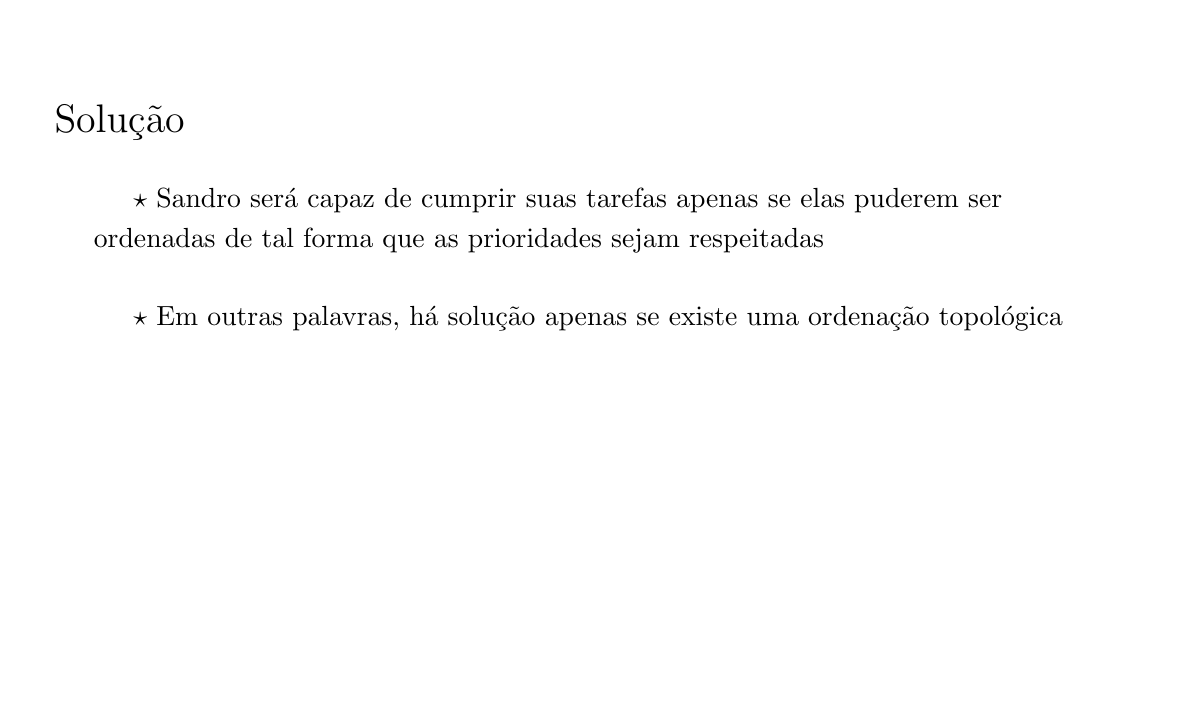
\begin{tikzpicture}
\node[draw,opacity=0] at (0, 0) {x};
\node[draw,opacity=0] at (14, 8) {x};

	\node[anchor=west] (title) at (0.0, 7.0) { \Large \bbbold{Solução} };

	\node[anchor=west] (a) at (1.0, 6.0) { $\star$ \bbtext{Sandro será capaz de cumprir suas tarefas apenas se elas puderem ser} };

	\node[anchor=west] (a1) at (0.5, 5.5) { \bbtext{ordenadas de tal forma que as prioridades sejam respeitadas} };


	\node[anchor=west] (b) at (1.0, 4.5) { $\star$ \bbtext{Em outras palavras, há solução apenas se existe uma ordenação topológica} };

\end{tikzpicture}
\end{frame}
\begin{frame}[plain,t]
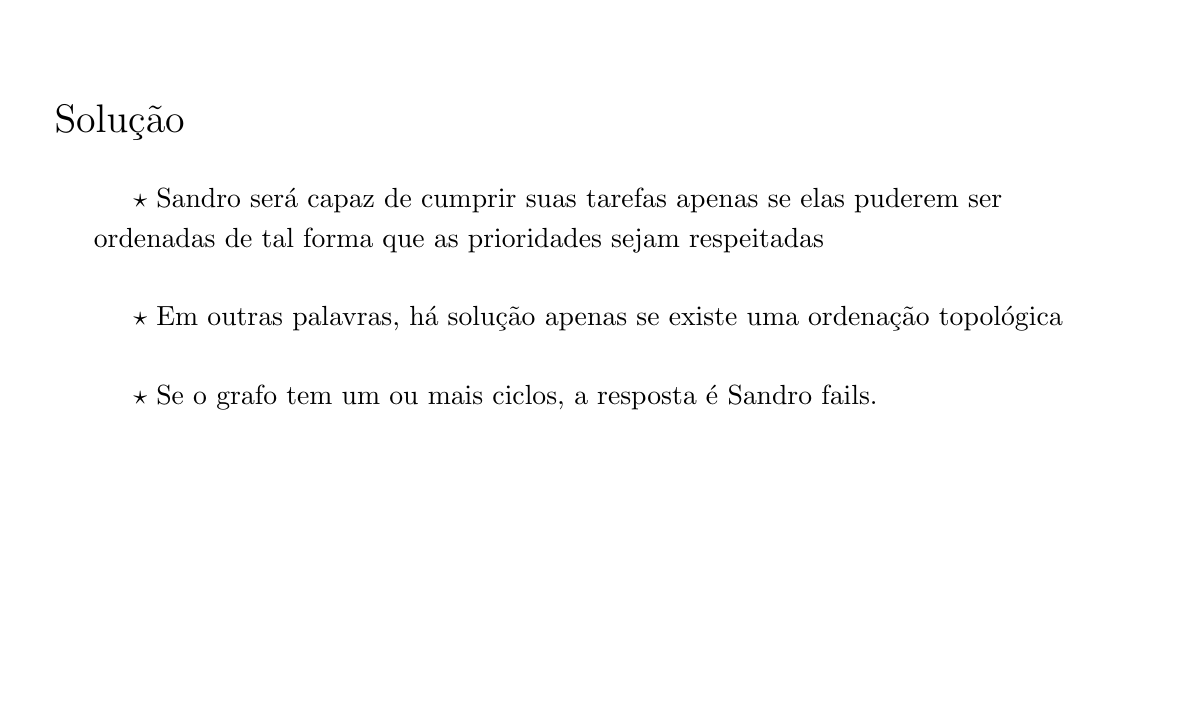
\begin{tikzpicture}
\node[draw,opacity=0] at (0, 0) {x};
\node[draw,opacity=0] at (14, 8) {x};

	\node[anchor=west] (title) at (0.0, 7.0) { \Large \bbbold{Solução} };

	\node[anchor=west] (a) at (1.0, 6.0) { $\star$ \bbtext{Sandro será capaz de cumprir suas tarefas apenas se elas puderem ser} };

	\node[anchor=west] (a1) at (0.5, 5.5) { \bbtext{ordenadas de tal forma que as prioridades sejam respeitadas} };


	\node[anchor=west] (b) at (1.0, 4.5) { $\star$ \bbtext{Em outras palavras, há solução apenas se existe uma ordenação topológica} };


	\node[anchor=west] (c) at (1.0, 3.5) { $\star$ \bbtext{Se o grafo tem um ou mais ciclos, a resposta é \bboutput{Sandro fails.}} };

\end{tikzpicture}
\end{frame}
\begin{frame}[plain,t]
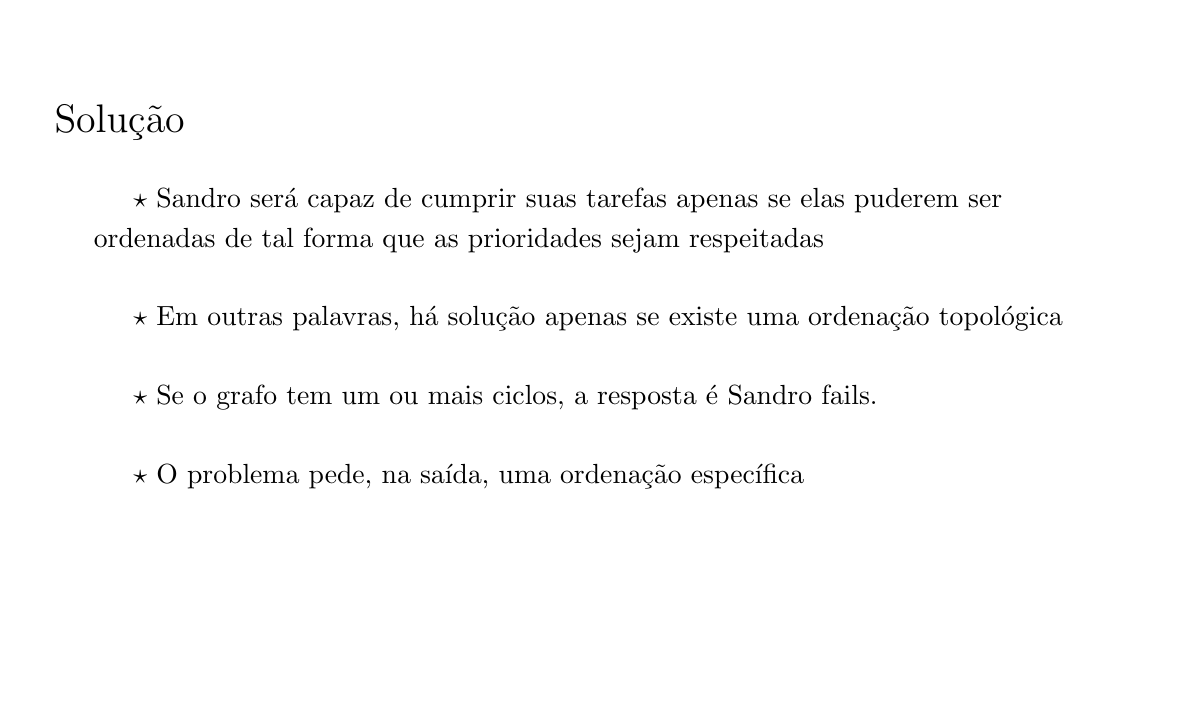
\begin{tikzpicture}
\node[draw,opacity=0] at (0, 0) {x};
\node[draw,opacity=0] at (14, 8) {x};

	\node[anchor=west] (title) at (0.0, 7.0) { \Large \bbbold{Solução} };

	\node[anchor=west] (a) at (1.0, 6.0) { $\star$ \bbtext{Sandro será capaz de cumprir suas tarefas apenas se elas puderem ser} };

	\node[anchor=west] (a1) at (0.5, 5.5) { \bbtext{ordenadas de tal forma que as prioridades sejam respeitadas} };


	\node[anchor=west] (b) at (1.0, 4.5) { $\star$ \bbtext{Em outras palavras, há solução apenas se existe uma ordenação topológica} };


	\node[anchor=west] (c) at (1.0, 3.5) { $\star$ \bbtext{Se o grafo tem um ou mais ciclos, a resposta é \bboutput{Sandro fails.}} };


	\node[anchor=west] (d) at (1.0, 2.5) { $\star$ \bbtext{O problema pede, na saída, uma ordenação específica} };

\end{tikzpicture}
\end{frame}
\begin{frame}[plain,t]
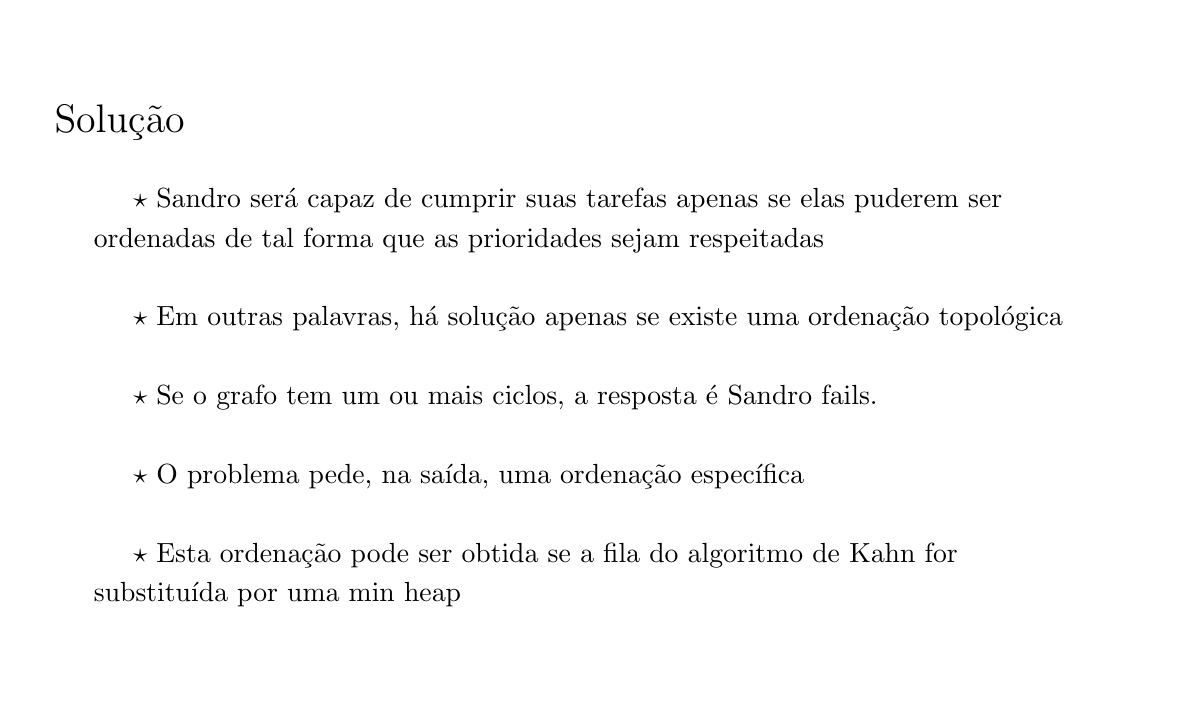
\begin{tikzpicture}
\node[draw,opacity=0] at (0, 0) {x};
\node[draw,opacity=0] at (14, 8) {x};

	\node[anchor=west] (title) at (0.0, 7.0) { \Large \bbbold{Solução} };

	\node[anchor=west] (a) at (1.0, 6.0) { $\star$ \bbtext{Sandro será capaz de cumprir suas tarefas apenas se elas puderem ser} };

	\node[anchor=west] (a1) at (0.5, 5.5) { \bbtext{ordenadas de tal forma que as prioridades sejam respeitadas} };


	\node[anchor=west] (b) at (1.0, 4.5) { $\star$ \bbtext{Em outras palavras, há solução apenas se existe uma ordenação topológica} };


	\node[anchor=west] (c) at (1.0, 3.5) { $\star$ \bbtext{Se o grafo tem um ou mais ciclos, a resposta é \bboutput{Sandro fails.}} };


	\node[anchor=west] (d) at (1.0, 2.5) { $\star$ \bbtext{O problema pede, na saída, uma ordenação específica} };


	\node[anchor=west] (e) at (1.0, 1.5) { $\star$ \bbtext{Esta ordenação pode ser obtida se a fila do algoritmo de Kahn for} };

	\node[anchor=west] (e1) at (0.5, 1.0) { \bbtext{substituída por uma \bbenglish{min heap}} };


\end{tikzpicture}
\end{frame}
\begin{frame}[plain,t]

\inputsnippet{cpp}{11}{29}{codes/TOPOSORT.cpp}

\end{frame}
\begin{frame}[plain,t]

\inputsnippet{cpp}{31}{42}{codes/TOPOSORT.cpp}


\end{frame}
\end{document}
